\section{Implementation and Evaluation Details}

The project ran in four phases. Phase 1 audited and de-duplicated the source
COCO data and froze a project-aware split. Phase 2 built the generation stack and
the augmented datasets. Phase 3 ran the controlled Mask R-CNN matrix and, after
the first single-seed pass proved uninformative, extended it to three seeds and
then to a rotated held-out cross-validation. Phase 4 tested whether the verdict
was backbone-dependent, first by fine-tuning SAM 3 and then by decomposing the
task into a class-agnostic detector plus a frozen DINOv2 classifier. The
ordering was not planned in advance; each phase was a response to what the
previous one failed to show.

\subsection{Insights derived from previous work}

Three readings of the prior literature shaped the design. First, Ghiasi et al.\
\cite{ghiasi2021copypaste} report that a crude pixel transplant with no
generative model beats more elaborate composition schemes. That result made a
non-generative control mandatory: without a copy-paste arm, any gain from
diffusion inpainting could equally be a gain from ``a rare polygon appears in a
new geometric context'', which has nothing to do with the generator. The
experiment matrix was therefore structured so that the diffusion treatment is
always flanked by a copy-paste control (identical pairing, identical target
polygon, zero generated pixels) and a deterministic feather-blend control
(identical pairing, seam smoothing but no diffusion).

Second, Fill-Up \cite{shin2023fillup} and DoGE \cite{wang2024doge} both
diagnose the same failure mode --- a frozen text-to-image model asked for an
out-of-distribution class produces images that do not lie in the target domain
--- and propose opposite fixes: adapt the generator (Fill-Up, via textual
inversion) or steer the frozen generator with a domain-gap embedding (DoGE). The
LoRA branch of this project implements the first of these on Stable Diffusion 1.5
inpainting \cite{rombach2022ldm,hu2022lora}. A preliminary qualitative check
confirmed the diagnosis was applicable: prompting the pretrained model with
``architectural technical floor plan, Versammlungsraum, 2D line drawing''
produced perspective furniture and photographic texture inside the masked room
rather than 2D symbols, visible in the right-hand panels of
Figure~\ref{fig:qastrategya} and Figure~\ref{fig:loraval}.

Third, and decisively, the literature evaluates these methods in a regime with
two to three orders of magnitude more data. LVIS \cite{gupta2019lvis} defines a
rare category as one appearing in fewer than 10 of about 100k training images;
our rare categories appear 3--8 times in a 35-image training split, and are tested
on 1--6 instances each. This is what motivated the class-agnostic track and,
later, the cross-validation and the two-stage decomposition: if a null result
was going to be reported, it had to be accompanied by evidence about
\emph{why} it was null, and about whether the measurement itself was capable of
detecting an effect.

\subsection{Technologies used}

Table~\ref{tab:tech} lists the main components. PyTorch and torchvision were
chosen for the detector because \protect\path{maskrcnn_resnet50_fpn_v2} provides a
well-understood, pretrained instance-segmentation baseline that trains on a
single GPU with a 35-image training set --- the point of the baseline is that it
is unremarkable, so that any measured difference is attributable to the data.
Hugging Face \texttt{diffusers} supplies the Stable Diffusion 1.5 inpainting
pipeline, whose nine-channel mask conditioning is what makes bit-exact
preservation outside the edited region possible. \texttt{peft} provides the LoRA
implementation. SAM 3 was run through Meta's own training harness rather than a
reimplementation, so that the comparison is against the model as its authors
configured it. DINOv2-base was loaded through \texttt{transformers} and used
strictly as a frozen feature extractor. Shapely handles polygon clipping when
crops are cut out of a plan, and \texttt{pycocotools} computes every AP reported
in this report, so that all numbers use the standard COCO definition
\cite{lin2014coco}.

\begin{table}[H]
\centering
\caption{Main technologies and their role in the project.}
\label{tab:tech}
\footnotesize
\begin{tabular}{@{}p{0.26\textwidth}p{0.30\textwidth}p{0.36\textwidth}@{}}
\toprule
Component & Version / identifier & Role \\
\midrule
PyTorch + torchvision & 2.1.2 (env \texttt{inpainting}) & Mask R-CNN training and evaluation \\
Mask R-CNN & \protect\path{maskrcnn_resnet50_fpn_v2}, ImageNet & baseline detector, both tracks \\
Stable Diffusion 1.5 inpainting & rev.\ \texttt{8a4288a7} & Strategy A/B/C generators \\
\texttt{diffusers}, \texttt{peft} & pinned in \texttt{requirements.txt} & diffusion pipeline, rank-8 LoRA \\
SAM 3 & \protect\path{facebookresearch/sam3} (env \texttt{sam3}, torch 2.10) & foundation-model detector \\
DINOv2-base & \texttt{facebook/dinov2-base} & frozen crop encoder, stage 2 \\
\texttt{pycocotools} & --- & COCO bbox/mask AP for every result \\
Shapely & --- & polygon clipping for rare-centred crops \\
Slurm & DFKI Pegasus cluster, A100/H100 & job orchestration \\
\bottomrule
\end{tabular}
\end{table}

\subsection{Student's contribution}

The pretrained weights (ImageNet, Stable Diffusion 1.5 inpainting, SAM 3,
DINOv2-base), the SAM 3 training harness, and the source COCO annotation file
are existing work. Everything else in the repository was designed and
implemented by the author: the Phase-1 audit and SHA-256 de-duplication; the
seeded project-aware split search; the safe-mask construction that erodes a room
polygon, subtracts overlapping annotations and protects detected dark strokes;
all three generation strategies and the LoRA training and conversion scripts;
the automated quality-control rules and the immutable decision audit; the
experiment runner with its fixed optimizer-step budget and provenance check that
rejects any augmented image not traceable to a training-split identifier; the
bounded rare-aware sampler; the class-agnostic dataset view; the SAM 3
configuration and the two bug fixes described in
Section~\ref{sec:problems}; the rotated held-out cross-validation; the DINOv2
feature extraction and two-stage evaluation; and the analysis scripts that
produce every table and figure in this report. The interpretation, the
statistical protocol and the decision to report a null result are likewise the
author's.

\subsection{Dataset Description and preprocessing}
\label{sec:dataset}

The source is a COCO-format collection of German fire-brigade floor plans
(\protect\path{area_segmentation_coco}) with 60 images, 1709 polygon annotations and
19 room categories. A Phase-1 audit verified that every referenced image file
exists and that every annotation is a valid polygon. SHA-256 comparison of the
image bytes identified four exact duplicates (COCO image IDs 22, 24, 25 and 26),
which were removed from the annotation file; the source JPEGs were left
untouched. The working dataset is therefore 56 images with 1633 annotations
over 19 categories, with model labels $1\ldots19$ and background $0$.

The plans come from 12 distinct building projects, and several plans of the same
project are near-identical floors of the same building. A random image-level
split would therefore place near-duplicates of the same floor on both sides of
the split. The split was instead generated by a seeded search over project-level
assignments, subject to the constraint that no project may contribute images to
more than one partition, and scored on how well it preserved rare-class coverage
in the test partition. The resulting frozen split assigns 35 images to train
(projects P01, P03, P05, P06, P08, P10--P13), 10 to validation (P02) and 11 to
test (P04, P07). It deviates from a 70/15/15 target in favour of valid rare-class
test coverage, which was judged the more useful property.

\begin{table}[H]
\centering
\caption{Per-class instance counts in the frozen project-aware split.
Categories 11--16 are the primary-rare group, 17--18 are low-support, and
category 19 has zero test instances and is excluded from all quantitative
claims. Source: \protect\path{outputs/splits/class_distribution_by_split.csv}.}
\label{tab:classdist}
\small
\begin{tabular}{@{}rlrrrr@{}}
\toprule
ID & Category & Train & Val & Test & Total \\
\midrule
1  & B\"uroraum            & 155 & 117 & 102 & 374 \\
2  & WC                    & 170 & 53  & 33  & 256 \\
3  & Treppe                & 117 & 38  & 57  & 212 \\
4  & Lager                 & 87  & 44  & 55  & 186 \\
5  & Technikraum           & 113 & 29  & 36  & 178 \\
6  & Aufzug                & 128 & 1   & 13  & 142 \\
7  & Andere                & 38  & 18  & 22  & 78  \\
8  & K\"uche               & 17  & 16  & 16  & 49  \\
9  & Flur, Halle           & 8   & 30  & 3   & 41  \\
10 & Besprechungsraum      & 16  & 8   & 11  & 35  \\
\midrule
11 & Allg.\ Verkehrsfl\"ache & 3 & 12  & 1   & 16  \\
12 & Abstellraum           & 8   & 1   & 2   & 11  \\
13 & Versammlungsraum      & 8   & 0   & 5   & 13  \\
14 & Schacht               & 3   & 7   & 2   & 12  \\
15 & Garderobe             & 4   & 0   & 6   & 10  \\
16 & Sanit\"arraum         & 4   & 3   & 1   & 8   \\
\multicolumn{2}{@{}l}{\emph{primary-rare subtotal}} & 30 & 23 & \textbf{17} & 70 \\
\midrule
17 & Werkstatt             & 4   & 0   & 1   & 5   \\
18 & Speiseraum            & 1   & 1   & 2   & 4   \\
19 & Labor                 & 3   & 0   & 0   & 3   \\
\midrule
\multicolumn{2}{@{}l}{\textbf{All categories}} & \textbf{887} & \textbf{378} & \textbf{368} & \textbf{1633} \\
\bottomrule
\end{tabular}
\end{table}

Figure~\ref{fig:classdist} shows the same distribution graphically and
Figure~\ref{fig:raresupport} isolates the tail. The consequence that governs the
whole report is in the ``Test'' column: the six primary-rare categories are
scored on 17 instances in total, and three of them on two instances or fewer. A
COCO AP computed over one or two instances is a step function; it cannot express
a small improvement.

\begin{figure}[H]
\centering
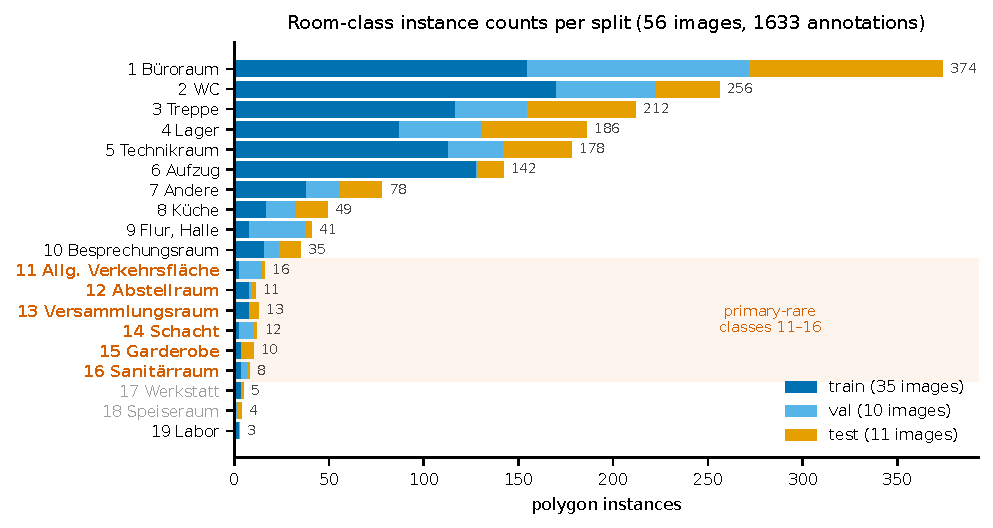
\includegraphics[width=\textwidth]{images/fig_class_distribution.pdf}
\caption{Room-class instance counts per split.}
\label{fig:classdist}
\end{figure}

\begin{figure}[H]
\centering
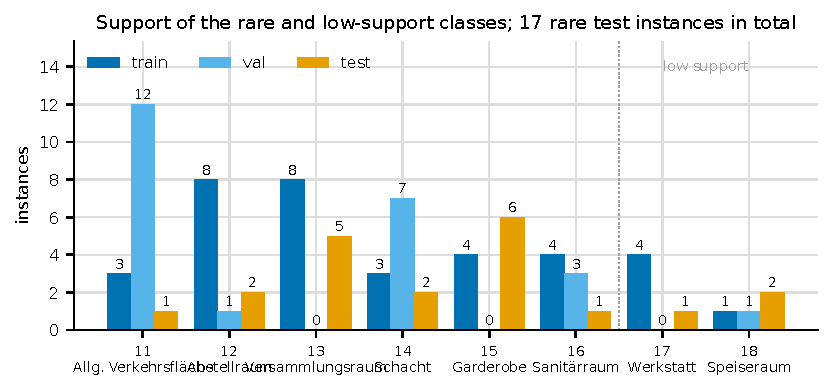
\includegraphics[width=\textwidth]{images/fig_rare_support.pdf}
\caption{Support of the rare and low-support classes.}
\label{fig:raresupport}
\end{figure}

A second view of the same data was derived for the class-agnostic track. It
preserves all 56 image records, all 1633 annotation identifiers, polygons,
bounding boxes and areas, and the frozen split, and rewrites every category to a
single foreground class \texttt{room}. The detector then has two classes instead
of twenty. Because the two views differ only in the label field, a difference
between the tracks is a difference between ``finding rooms'' and ``naming
rooms''.

\subsubsection*{Generation strategies}

All generators read the frozen training image identifiers and nothing else; the
loader traces every augmented image back to a training identifier and rejects
validation or test provenance rather than silently filtering. Three strategies
were implemented.

\emph{Strategy A} converts a real rare room into a different appearance of the
same rare class. The room polygon is rasterised at original resolution, eroded
by $\mathrm{round}(\mathrm{clamp}(0.02\cdot\min(w,h),2,12))$ pixels to protect
its walls, intersected against all overlapping annotations, and dark strokes
detected by Otsu thresholding inside the room are dilated by two pixels and
protected. Only the resulting safe mask is editable. A crop with one bounding-box
width and height of context on each side is white-padded and resized to $512^2$,
inpainted, inverse-mapped, and composited back through the original-resolution
safe mask. The written PNG is reopened and compared against the source: exact
invariance outside the safe mask is mandatory and cannot be disabled by
configuration. Figure~\ref{fig:qastrategya} shows the seven-panel audit row
produced for every candidate.

\emph{Strategy B} converts a \emph{common} room into a rare one. Common classes
1--10 are screened against the real rare-class ranges of area, aspect ratio,
width, height and polygon solidity (5th--95th percentile expanded by 50\%), each
source annotation is used at most once, and the per-class target is
$\min(3 \times n_{\mathrm{real}}, 20)$. Only the selected annotation's category
label changes; its polygon and every other annotation stay as they are.

\emph{Strategy C} is exemplar-guided. Instead of asking the model to invent a
rare room, a real rare training room is transplanted into a geometry-compatible
common-room polygon: both polygons are rasterised, the target interior is
cleared, the donor bounding box and mask are affinely mapped onto the target, and
only donor pixels are inserted. Diffusion is then restricted to a narrow inner
seam and to editable target pixels the warped donor does not cover, at strength
0.30 --- the core donor pixels lie outside the diffusion mask by construction.
Three modes were generated from the identical pairing plan so that the diffusion
contribution is isolated: C0 direct copy-paste (no generated pixels, arm e8), C1
deterministic feather blending (arm e9), and C2 exemplar-seeded diffusion
inpainting (arms e10/e11). Figure~\ref{fig:qastrategyc} shows a C0 audit row.

\emph{The LoRA branch} trains one shared rank-8 adapter on the attention
projections of the SD 1.5 inpainting U-Net, freezing the VAE, text encoder and
base U-Net. Training crops are room-centred $512^2$ crops from training
annotations only, with 12 deterministic classical variants per usable rare crop
(brightness, contrast, grayscale, mild blur, scan noise, line-thickness and a
small geometry-aligned affine); those variants share a
\protect\path{source_annotation_id} and are explicitly recorded as \emph{not}
independent geometries. The prompt template is ``architectural technical floor
plan, \{category\_name\}, 2D line drawing''. The trained adapter then drives a
Strategy-B-style common-to-rare conversion (arms e12/e13).
Figure~\ref{fig:loraval} is the fixed-seed validation contact sheet comparing
pretrained SD against the adapter on the same source, mask and seed.

Acceptance is fully automatic and auditable. A candidate is rejected for an
empty or too-small editable region, a near-identical or blank or uniform output,
an extreme increase in dark or saturated fill, a safety-checker flag, any changed
pixel outside the editable interior or on the protected boundary, or a hash
mismatch on the written file. Table~\ref{tab:acceptance} reports the outcome.
These are raster checks only: they certify that the surrounding drawing is
untouched and that the edited region is not degenerate, but they cannot certify
that the generated interior depicts the requested room type. Every strategy's
metadata therefore records \protect\path{semantic_correctness = unverified}, except
Strategy C, which records \protect\path{real_train_exemplar_preserved} because its
rare pixels are copied from a real annotated room of that class.

\begin{table}[H]
\centering
\caption{Automated acceptance of generated candidates, per generation branch.
Sources: \protect\path{outputs/augmentation_a/summary.json},
\protect\path{augmentation_b/summary.json}, \protect\path{augmentation_c/*/summary.json},
\protect\path{augmentation_lora_b/summary.json}. ``Rare geometries added'' counts
common-room polygons relabelled to a rare class; for Strategy A the edit changes
the appearance of an existing rare room, so no new rare polygon is created.}
\label{tab:acceptance}
\small
\begin{tabular}{@{}llrrrl@{}}
\toprule
Branch & Arms & Attempted & Accepted & Rate & Dominant rejection reasons \\
\midrule
A (prompt, rare$\rightarrow$rare)   & e2--e5   & 90 & 74 & 0.82 & extreme dark filling (14) \\
B (prompt, common$\rightarrow$rare) & e6--e7   & 40 & 27 & 0.68 & safe mask too small (8) \\
C0 copy-paste                       & e8       & 52 & 46 & 0.88 & editable region too small (5) \\
C1 feather blend                    & e9       & 52 & 45 & 0.87 & editable region too small (5) \\
C2 diffusion inpaint                & e10--e11 & 52 & 45 & 0.87 & editable region too small (5) \\
LoRA (prompt, common$\rightarrow$rare) & e12--e13 & 52 & 31 & 0.60 & generated region uniform (10) \\
\bottomrule
\end{tabular}
\end{table}

\begin{figure}[H]
\centering
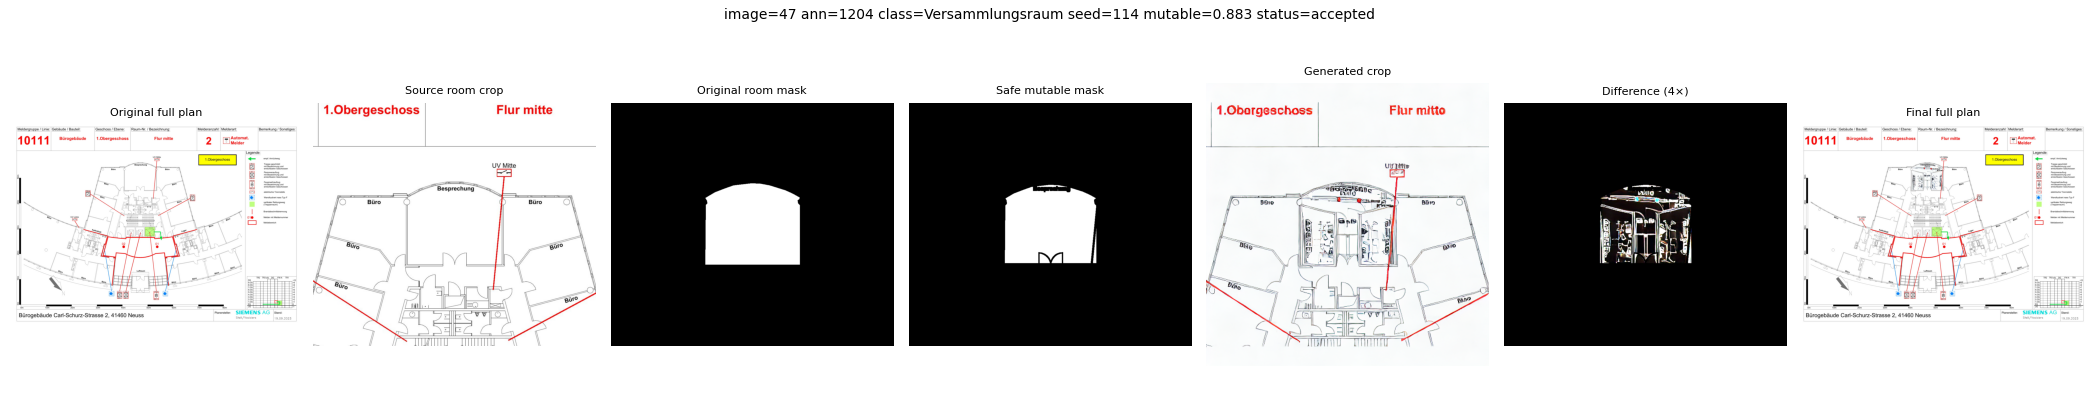
\includegraphics[width=\textwidth]{images/strategy_a_row.png}
\caption{Strategy A quality-control audit row (accepted candidate).}
\label{fig:qastrategya}
\end{figure}

The Strategy A row in Figure~\ref{fig:qastrategya} is worth reading closely,
because it shows both that the safety machinery works and that the semantics do
not. The ``Difference'' panel is confined entirely to the safe mask, so the
surrounding plan is bit-identical --- but the ``Generated crop'' contains
perspective furniture and photographic shading, not the 2D symbols of a German
Versammlungsraum. This candidate passed every automated check and entered the
training set.

\begin{figure}[H]
\centering
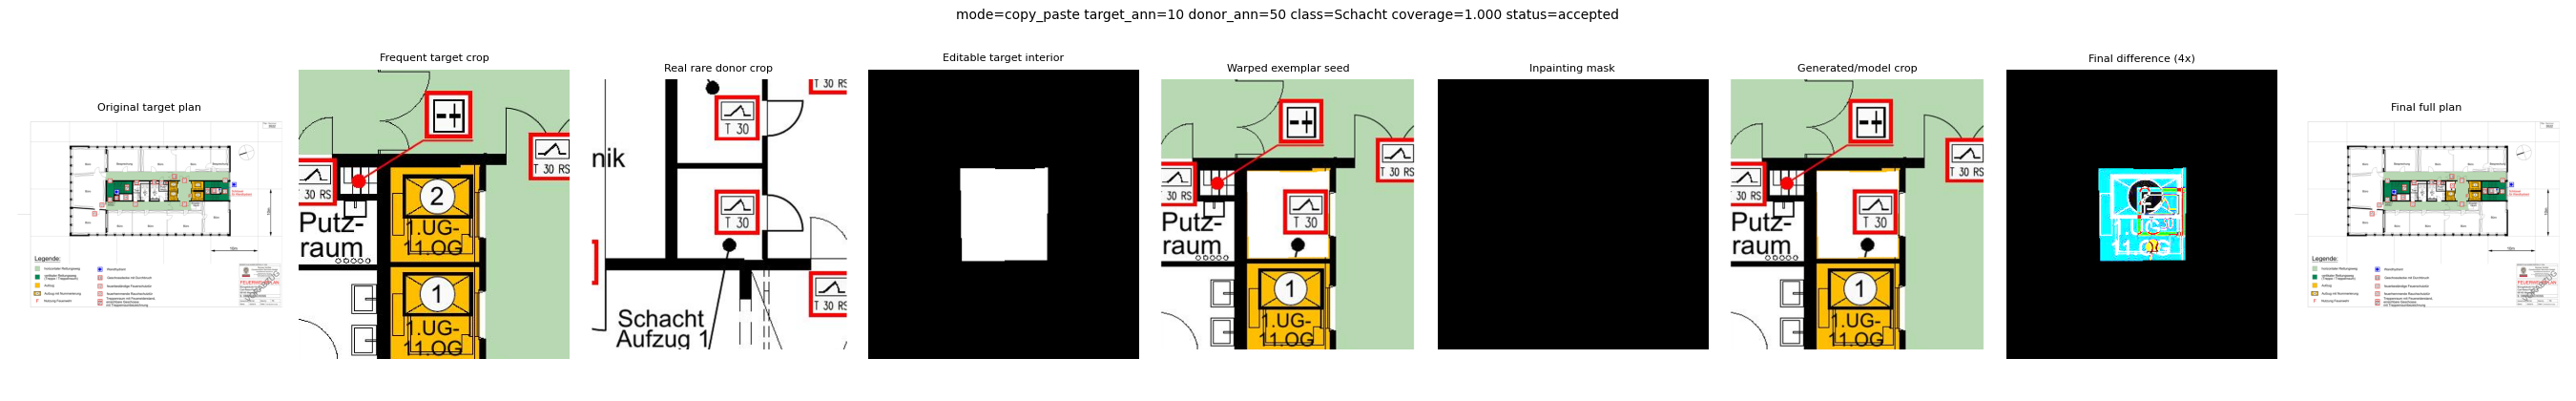
\includegraphics[width=\textwidth]{images/strategy_c_copypaste_row.png}
\caption{Strategy C exemplar copy-paste audit row.}
\label{fig:qastrategyc}
\end{figure}

\begin{figure}[H]
\centering
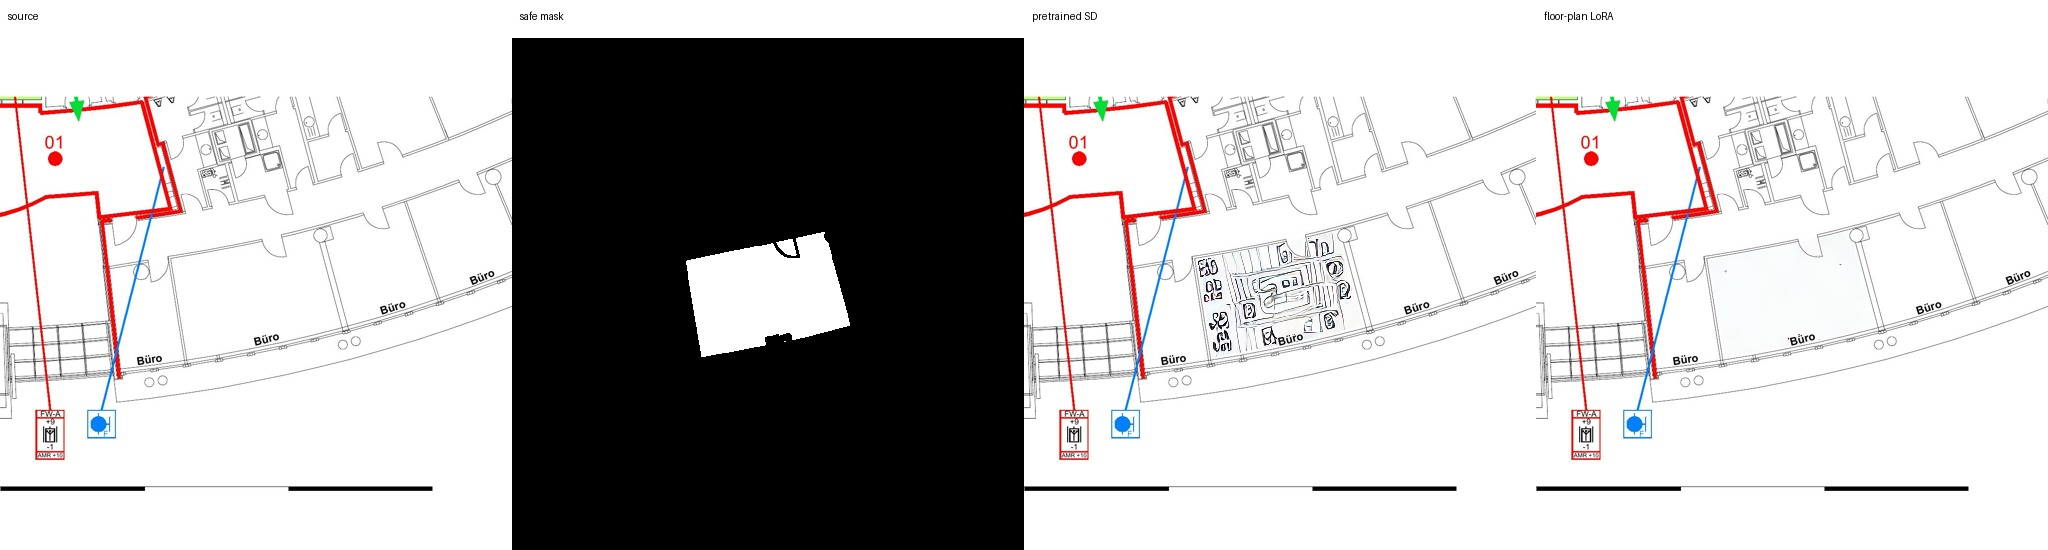
\includegraphics[width=\textwidth]{images/lora_val_13.jpg}
\caption{Pretrained Stable Diffusion versus the floor-plan LoRA on a fixed case.}
\label{fig:loraval}
\end{figure}

Figure~\ref{fig:loraval} isolates what the adapter learned. Given the same
source, safe mask and seed, pretrained SD (third panel) fills the room with
dense pseudo-furniture, while the LoRA (fourth panel) produces a nearly empty
light-grey region. The adapter successfully learned that floor plans are mostly
white space --- and, because the mask construction protects detectable dark
strokes, it was largely trained on regions from which the strongest category cues
had already been removed. The result is safe and domain-consistent output that
carries no room-type information, which is a plausible mechanism for the
downstream measurements in Section~\ref{sec:results}.

\subsection{Experimental Setup and Evaluation}

Every experiment reports COCO bbox and mask AP computed by \texttt{pycocotools}
against the untouched test annotations \cite{lin2014coco}. The multiclass track
additionally reports a rare-macro mask AP, defined as the unweighted mean over
categories 11--16 that have non-zero test support. The class-agnostic track
reports overall \texttt{room} AP; rare-macro AP is undefined there. Augmented
data is used for training only; validation and test always use the original
held-out images and annotations.

\subsubsection{Goal 1: the controlled experiment matrix}

Fourteen arms were defined, listed in Table~\ref{tab:arms}. Each arm declares
both tracks, and each is trained from independent ImageNet initialisation with
the identical recipe: \protect\path{maskrcnn_resnet50_fpn_v2}, 25 epochs, exactly 35
optimizer steps per epoch, SGD at learning rate 0.005 with momentum 0.9 and
weight decay $5\times10^{-4}$, a step schedule dropping by $0.1$ every 8 epochs,
batch size 1, aspect-preserving resize with \texttt{min\_size} 1024 and
\texttt{max\_size} 1600, AMP, and horizontal flip plus mild photometric jitter.
Fixing the optimizer-step budget rather than the epoch count over a larger
dataset is what makes the arms comparable: an augmented arm sees a different
\emph{mixture} of images than e0, but not more gradient updates. The best
checkpoint is selected on validation mask AP.

The rare-aware sampler used by the ``$+$w'' arms assigns each training image the
bounded weight
\[
  w_i \;=\; \min\!\left(5,\; 1 + 2\sum_c \frac{n_{ic}}{\sqrt{n^{\mathrm{real}}_c}}\right),
\]
where $n_{ic}$ counts instances of class $c$ in image $i$ and
$n^{\mathrm{real}}_c$ is the class count in the \emph{original} training
annotations, so that synthetic images cannot inflate their own weight. The cap
bounds any single image's sampling probability.

\begin{table}[H]
\centering
\caption{The fourteen controlled arms. ``$+$w'' denotes bounded rare-aware image
sampling; ``$+$crop'' mixes rare-centred crops with full plans at probability
$0.4/0.6$. Every arm runs both the multiclass and the class-agnostic track.}
\label{tab:arms}
\small
\begin{tabular}{@{}llll@{}}
\toprule
Arm & Training data & Sampling & Role \\
\midrule
e0  & original 35 plans                & uniform & baseline \\
e1  & original 35 plans                & rare-weighted & sampling-only control \\
e2  & $+$ Strategy A                   & uniform & prompt inpainting, rare$\rightarrow$rare \\
e3  & $+$ Strategy A                   & rare-weighted & A $\times$ sampling \\
e4  & $+$ Strategy A $+$ crops         & uniform & A $\times$ crop mixing \\
e5  & $+$ Strategy A $+$ crops         & rare-weighted & A $\times$ crops $\times$ sampling \\
e6  & $+$ Strategy B                   & uniform & prompt inpainting, common$\rightarrow$rare \\
e7  & $+$ Strategy B                   & rare-weighted & B $\times$ sampling \\
e8  & $+$ Strategy C0 copy-paste       & uniform & \emph{non-generative control} \\
e9  & $+$ Strategy C1 feather blend    & uniform & deterministic-blending control \\
e10 & $+$ Strategy C2 diffusion inpaint& uniform & \emph{primary inpainting treatment} \\
e11 & $+$ Strategy C2 diffusion inpaint& rare-weighted & C2 $\times$ sampling \\
e12 & $+$ LoRA Strategy B              & uniform & adapted-generator treatment \\
e13 & $+$ LoRA Strategy B              & rare-weighted & LoRA $\times$ sampling \\
\bottomrule
\end{tabular}
\end{table}

Goal 1 is verified rather than scored: all generators were confirmed to read only
frozen training identifiers, every accepted sample carries a recorded
quality-control decision and output hash, and every arm ran both tracks under the
identical budget. Table~\ref{tab:acceptance} is the corresponding evidence.

\subsubsection{Goal 2: the three-seed grid and the rotated held-out cross-validation}

The grid runs all 14 arms $\times$ 2 tracks $\times$ 3 seeds $\{42, 123, 2026\}$,
for 84 training runs. Per-arm results are the mean and population standard
deviation over the three seeds. Each augmented arm is compared to e0 by a paired
test over the seeds --- Wilcoxon signed-rank where applicable, falling back to an
exact two-sided sign test. At $n=3$ the smallest attainable two-sided sign-test
$p$-value is $0.25$, which occurs only when all three seed-level differences share
a sign; this ceiling is a property of the design and is stated with every
$p$-value in Section~\ref{sec:results}.

The single-seed pass that preceded the grid produced apparently large effects
(for example, Strategy A at $0.121$ multiclass mask AP against $0.075$ for e0 on
seed 42 alone) that did not survive the addition of two further seeds. That
experience is why no single-seed number is treated as evidence anywhere in this
report.

The grid's weakness is the 11-image test split. The rotated held-out
cross-validation addresses it without retraining anything. The 35-image training
split is held fixed for every fold --- so the augmented datasets, which are built
from that split, and all grid checkpoints remain valid --- and only the
evaluation set rotates: the 21 held-out images (validation $+$ test) are
partitioned round-robin into $K=5$ folds, and each frozen checkpoint is
re-evaluated on each fold in evaluation-only mode. Across the folds every
held-out image is tested exactly once, and the pooled rare test support rises
from 17 to 40 instances. Six arms $\{$e0, e1, e6, e8, e10, e12$\}$ were selected
to span the families, giving $6 \times 2 \times 5 = 60$ evaluations. The
project-aware constraint is not violated: the 21 held-out images span only three
projects, so a project-aware $K>3$ partition is impossible, but the only leakage
that could matter --- between the frozen training split and the evaluation images
--- is prevented by construction because no fold trains anything. Per-fold
paired tests against e0 use the same sign-test protocol; at $K=5$ the minimum
attainable two-sided $p$-value is $0.0625$.

\subsubsection{Goal 3: SAM 3}

SAM 3 \cite{carion2025sam3} was fine-tuned with Meta's official trainer on the
unchanged split, using the 19 German category names as text concepts for the
multiclass track and a single \texttt{room} concept for the class-agnostic track.
The configuration is 20 epochs at resolution 1008, AdamW with gradient clipping
at max-norm 0.1, layer-wise learning-rate decay of 0.9 on the vision trunk, and
three learning-rate groups on an inverse-square-root schedule --- $8\times10^{-5}$
for the heads, $2.5\times10^{-5}$ for the vision backbone and $5\times10^{-6}$
for the language backbone --- with instance-mask loss and the model's presence
head enabled at evaluation. Evaluation writes COCO prediction JSON and is scored
with the same \texttt{pycocotools} path as the Mask R-CNN runs, so the two
backbones' numbers are directly comparable.

Three augmentation datasets were carried across verbatim, without regeneration:
Strategy C2 diffusion inpaint (the e10 data), LoRA Strategy B (the e12 data) and
Strategy C0 copy-paste (the e8 data). Each was run once per track, giving a
baseline plus three augmented runs in each of the two tracks. These are
single-seed runs; the seed-to-seed standard deviation measured on the grid is the
noise floor against which their deltas must be read, and Section~\ref{sec:results}
does exactly that.

\subsubsection{Goal 4: the two-stage DINOv2 pipeline}

The two-stage pipeline is drawn in Figure~\ref{fig:pipeline}. Stage 1 is the
already-trained class-agnostic SAM 3 detector, which contributes 483 test
proposals. Each proposal or annotation bounding box is expanded by a context
margin, clamped to the image, padded to a white square and resized to $224^2$.
Stage 2 encodes the crop with a frozen DINOv2-base \cite{oquab2024dinov2} and
represents it by the concatenation of the CLS token and the mean of the patch
tokens, a 1536-dimensional vector; features are standardised and
$\ell_2$-normalised. Two heads were trained on those features: a linear
classifier (Adam, 300 epochs, inverse-square-root class weighting) and a cosine
$k$-NN with $k=5$. No gradient reaches the backbone in either case.

\begin{figure}[H]
\centering
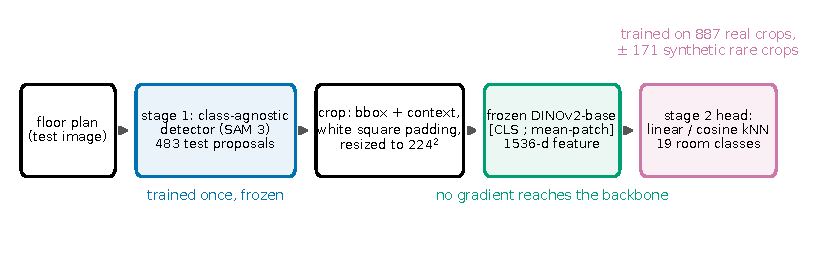
\includegraphics[width=\textwidth]{images/fig_twostage_pipeline.pdf}
\caption{The two-stage room-typing pipeline.}
\label{fig:pipeline}
\end{figure}

Two arms differ only in the head's training set: \texttt{real} uses the 887 real
training-split ground-truth crops, and \texttt{real\_plus\_synth} adds the 171
rare crops produced by the augmentation pipeline. Two evaluations are reported.
Evaluation A classifies the 368 real ground-truth test crops, which removes
detector error entirely and therefore measures the classification bottleneck in
isolation; it reports top-1 accuracy, head-macro recall over classes 1--10 and
rare-macro recall over 11--16. Evaluation B labels the 483 class-agnostic test
proposals with the head and scores the result as multiclass instance
segmentation with \texttt{COCOeval(segm)} against the multiclass test ground
truth, which puts the two-stage system on exactly the same axis as the
end-to-end fine-tuned detectors.

\subsection{Ethical considerations}

The dataset contains architectural drawings of real, identifiable buildings ---
specifically fire-brigade plans, which mark escape routes, hydrants and shafts.
It contains no personal data and no images of people, so the privacy exposure is
institutional rather than individual, but the plans are not public documents and
were not redistributed. All diffusion inference ran locally on cluster nodes
against a pre-downloaded model cache with Hugging Face offline mode enabled, so
no floor-plan image was transmitted to a third-party service at any point. The
Stable Diffusion safety checker was retained rather than disabled; it flagged and
rejected a small number of candidates (two in Strategy A, two in C2, two in the
LoRA branch), which were discarded like any other rejection.

The clearest ethical risk in the work is the synthetic data itself. The
generation pipeline produces images that look like genuine fire-brigade plans but
in which a room has been silently relabelled --- a Technikraum redrawn and
annotated as a Schacht. Such an image is safe as a training sample and unsafe as
a document: if it escaped the training directory it could be mistaken for a real
plan of a real building, with obvious consequences for anyone relying on it in an
emergency. The pipeline mitigates this by construction rather than by convention:
synthetic images live in separate \protect\path{data/augmented_*} directories, carry a
\texttt{strategy} field and a stable synthetic identifier in their COCO records,
and are never written back into the source dataset, which remains byte-identical
throughout. This report reproduces synthetic panels only inside labelled
quality-control figures.

A second concern is honest reporting. Generation-side metadata records
\protect\path{semantic_correctness = unverified} wherever automatic checks cannot
establish that a generated region depicts the requested class, and the file
\protect\path{outputs/augmentation_b/review.csv} is explicitly an automatic decision
audit rather than a human review gate. Related to this, the LoRA branch
documentation records that the prompt-only conversion retained visible
common-room text labels such as ``B\"uro'' in some accepted samples; the e12/e13
results are reported here as measurements of that data as it was actually used,
with the caveat stated, rather than quietly dropped. The project's central claim
is a negative one, and it is reported as such --- with $n$, standard deviation
and $p$-value --- rather than being narrowed to the subset of arms and metrics
that happen to look favourable.

\subsection{Reproducibility and code availability}

All code, configuration, tests and documentation are in a single Git repository
at commit \texttt{d1b08f0}; datasets, model weights and outputs are
machine-local and deliberately untracked. The cluster checkout lives in one
directory, \protect\path{/netscratch/espandar/inpainting/floorplan-inpainting/}, with
code in \texttt{src/}, \texttt{scripts/}, \texttt{slurm/} and \texttt{configs/},
derived datasets in \texttt{data/}, adapters in \texttt{models/} and every
result, checkpoint and log below \texttt{outputs/}. The consolidated summaries
that this report cites are in \texttt{outputs/final/}: \texttt{grid\_r1/},
\texttt{cv/}, \texttt{sam3/} and \texttt{dino/}, each holding a
\texttt{summary.json} and \texttt{summary.csv}.

Two conda environments are used because the two backbones have incompatible
requirements: \texttt{inpainting} (PyTorch 2.1.2) for data preparation, the
diffusion generators, Mask R-CNN and the DINOv2 stage, and \texttt{sam3}
(PyTorch 2.10) for SAM 3. Experiments run on the DFKI Pegasus Slurm cluster on
A100 and H100 nodes; SAM 3 jobs are pinned to the 80\,GB GPU tier. Four submit
scripts reproduce the whole set of results, each of them a dependency chain of
the form ``build inputs $\rightarrow$ smoke test one task $\rightarrow$ full array
$\rightarrow$ analyse'':

\begin{table}[H]
\centering
\caption{Reproduction entry points. Each script is run from the project
directory on the cluster and writes its consolidated result under
\texttt{outputs/final/}.}
\label{tab:repro}
\small
\begin{tabular}{@{}lll@{}}
\toprule
Script & Work & Output \\
\midrule
\protect\path{scripts/submit_grid_r1.sh}  & 14 arms $\times$ 2 tracks $\times$ 3 seeds & \protect\path{outputs/final/grid_r1/} \\
\protect\path{scripts/submit_cv.sh}        & 5-fold rotated held-out re-evaluation & \protect\path{outputs/final/cv/} \\
\protect\path{scripts/submit_sam3_aug.sh} & SAM 3 baseline $+$ 3 augmentations, 2 tracks & \protect\path{outputs/final/sam3/} \\
\protect\path{scripts/submit_dino.sh}      & DINOv2 extraction, heads and two-stage eval & \protect\path{outputs/final/dino/} \\
\bottomrule
\end{tabular}
\end{table}

Determinism is bounded and stated rather than promised. Split generation, seed
assignment, sampler construction, candidate ordering and quality-control
thresholds are fully deterministic, and every generated sample carries a stable
identifier, its seed, the exact model revision
(\texttt{8a4288a76071f7280aedbdb3253bdb9e9d5d84bb}), the LoRA weight hash and the
output file hash, so an interrupted run resumes by sample identifier and a
changed configuration is forced into a new output directory. Diffusion sampling
reproduces a given candidate on the same software and GPU stack, but bitwise
reproducibility across different GPU models is not claimed. Detector training
uses AMP and a fixed seed, and the seed-to-seed spread reported in
Section~\ref{sec:results} is precisely the residual variation this leaves.
The figures in this report are regenerated from the fetched summary files by
\protect\path{report/scripts/make_figures.py}, which is committed alongside them.

At the time of writing the repository has not been pushed to a public forge, so
the cluster checkout is synchronised in place from the local \texttt{main}
branch by \protect\path{scripts/deploy_cluster.sh}, which ships the history as a Git
bundle and fast-forwards the remote checkout. Once a hosted remote is
configured this is replaced by an ordinary \texttt{git pull} and the bundle
mechanism can be deleted. Code availability to a third party is therefore
currently by request rather than by URL.

\subsection{Problems faced during the project}
\label{sec:problems}

\emph{The test split is too small to measure the thing the project is about.}
This is the fundamental problem, and it was not solved. Six rare categories are
scored on 17 test instances, three of them on two instances or fewer. A COCO AP
over two instances takes a handful of discrete values, so a genuine small
improvement in rare-class segmentation is not representable, let alone
distinguishable from noise. Two mitigations were built --- three seeds, to
measure the noise, and the rotated cross-validation, to raise the pooled rare
support from 17 to 40 --- and both helped characterise the measurement without
removing the ceiling. The honest statement of the outcome is that the experiment
can exclude a large rare-class effect and cannot resolve a small one.

\emph{SAM 3 training bugs.} Two defects had to be found and fixed before any SAM 3
number existed. The first was silent: training ran, the loss printed as a
constant zero, and \texttt{loss.backward()} raised ``does not require grad''.
The cause is that the trainer resolves a loss module by the collate function's
\texttt{dict\_key}; any key it cannot match falls back to
\texttt{trainer.loss.default}, which is a \texttt{DummyLoss} returning a constant
with no \texttt{grad\_fn}. The training collate function must use
\texttt{dict\_key: all} so it resolves to the real \texttt{Sam3LossWrapper}, as
Meta's own training configurations do. The second appeared only at the first
validation epoch: with \texttt{enable\_segmentation} the validation dataset
yields RLE-encoded masks, and \protect\path{RandomResizeAPI.resize()} indexes
\texttt{obj.segment} as a tensor, so the job died with
\texttt{KeyError: (None, None)} after the training epochs had already been paid
for. The fix is to place \texttt{DecodeRle} before any geometric transform in
the validation pipeline. Both fixes are recorded as comments in
\protect\path{configs/sam3_floorplan.yaml} so they are not silently reverted.

\emph{Grid out-of-memory at \texttt{-{}-mem=32G}.} The first grid submission
requested 32\,GB of host memory per task and tasks were killed during data
loading rather than on the GPU: at \texttt{min\_size} 1024 / \texttt{max\_size}
1600 with several workers, the decoded full-resolution plans plus the augmented
COCO index exceed that budget. The request was raised to 64\,GB, which is
sufficient.

\emph{A resume bug that corrupted optimizer state.} Runs are restartable with
\texttt{-{}-resume}, and the resume path initially rebuilt the model \emph{without}
pretrained weights on the assumption that the checkpoint would supply them. It
does supply the weights, but constructing the model differently changes which
parameters are trainable, so the parameter groups no longer matched the saved
optimizer state and \protect\path{optimizer.load_state_dict} failed --- or, worse,
matched positionally and restored momentum buffers onto the wrong tensors. The
model construction was made identical on the resume path and the fresh path, and
the run's configuration fingerprint is now checked before a resume is allowed.

\emph{Queue latency on the 80\,GB tier.} SAM 3 at resolution 1008 requires an
80\,GB GPU, and \protect\path{sam3_aug.sbatch} is restricted to the
A100-80GB/H100/H200 partitions. Those partitions are the most contended on the
cluster, so wall-clock turnaround for a six-task array was dominated by queueing
rather than by compute. The practical mitigation was structural: every submit
script begins with a single cheap smoke task and makes the full array depend on
\texttt{afterok}, so a configuration error costs one queued task rather than a
full array's worth of allocations. This is also why the SAM 3 comparison is
single-seed --- a three-seed SAM 3 grid was not affordable in queue time, and
that limitation is carried explicitly into the interpretation of its results.

\emph{Invalidated LoRA generation data.} Quality-assurance inspection of the
prompt-only LoRA conversion showed that some accepted samples retained the
original common-room text label (for example ``B\"uro'' still printed inside a
room now annotated as a rare class), because the mask construction protects
detected dark strokes and therefore protects exactly the labels that identify the
old class. A revised ``semantic v2'' generator was implemented that masks compact
interior labels while preserving structural lines and seeds generation with a
real rare exemplar. The e12/e13 grid arms and the SAM 3 LoRA-b run reported here
use the original prompt-only data, so they are best read as evidence about that
generator rather than about class-conditioned LoRA inpainting in general.
